\newpage
\begin{center}
  \textbf{\large 1 АНАЛИЗ ПРЕДМЕТНОЙ ОБЛАСТИ И ТЕХНОЛОГИЙ}
\end{center}

\addcontentsline{toc}{section}{1 АНАЛИЗ ПРЕДМЕТНОЙ ОБЛАСТИ И ТЕХНОЛОГИЙ}

\textbf{\large 1.1 Предметная область}
\addcontentsline{toc}{subsection}{1.1 Предметная область}

Предметная область данной выпускной квалификационной работы связана с разработкой программного обеспечения для проектирования баз данных. Современные информационные технологии играют ключевую роль в управлении данными, что делает процесс проектирования баз данных важным этапом в разработке программного обеспечения. Компании, разработчики и аналитики нуждаются в удобных и гибких инструментах, которые позволяют создавать, редактировать и визуализировать структуры баз данных. При этом важным аспектом становится не только сам процесс проектирования, но и возможность генерации SQL-кода, обмена схемами и совместной работы над проектами.
	
На сегодняшний день существует множество инструментов для работы с базами данных, включая популярные решения, такие как dbdesigner, database-design, dbdiagram.io и другие. Однако большинство из них либо сложны в освоении для начинающих пользователей, либо ограничены в бесплатных версиях, либо не предоставляют возможности работать с DBML (Database Markup Language) — удобным языком разметки, который используется для текстового описания структуры базы данных.

В последние годы язык DBML набирает популярность благодаря своей читаемости, простоте использования и удобству при описании баз данных в текстовом формате. Однако несмотря на его преимущества, число инструментов, поддерживающих этот стандарт, остается ограниченным, а имеющиеся решения зачастую не предоставляют достаточно гибкости и функциональности для полноценной работы с базами данных.

Актуальность данной работы обусловлена отсутствием универсального инструмента, который бы позволял визуально проектировать базы данных, поддерживал DBML, автоматически генерировал SQL-код, а также обеспечивал удобство командного взаимодействия. В настоящее время пользователям приходится либо использовать несколько разрозненных инструментов, либо прибегать к сложным и дорогостоящим решениям, которые не всегда отвечают их требованиям.

Предметная область данной работы охватывает несколько ключевых направлений:

\begin{itemize}
    \item Разработка программного обеспечения для визуального проектирования баз данных — создание удобного интерфейса, в котором пользователи смогут наглядно создавать таблицы, указывать связи и определять структуру данных.
    \item Генерация кода в формате DBML и SQL, позволяющая экспортировать созданные схемы в удобном виде для последующего использования в различных СУБД.
    \item Интеграция функций командной работы, что актуально для небольших команд разработчиков, стартапов, студентов и аналитиков, которым необходимо совместно редактировать и обсуждать структуры баз данных.
\end{itemize}

Основная проблема, на решение которой направлена данная работа, заключается в создании удобного, интуитивно понятного и доступного инструмента для проектирования баз данных, который объединяет в себе визуальное редактирование схем, поддержку DBML, автоматическую генерацию SQL-кода и возможности командного взаимодействия. Такой продукт позволит значительно упростить процесс проектирования баз данных, сделает его более доступным для начинающих разработчиков, студентов и небольших команд, а также повысит удобство и скорость работы профессиональных архитекторов данных.

Разрабатываемое программное обеспечение ориентировано на широкий круг пользователей, включая разработчиков, студентов, стартапы, фрилансеров, аналитиков и архитекторов баз данных. В зависимости от потребностей, инструмент можно будет использовать в учебных целях,также как профессиональный инструмент для проектирования или платформу для совместной работы над схемами баз данных.

Целью разработки является создание универсального программного обеспечения, которое обеспечит интуитивно понятный интерфейс, поддержку DBML, автоматическую генерацию SQL-кода и возможности для командной работы. Это позволит упростить процесс проектирования баз
данных и сделать его более доступным для широкого круга пользователей.

\

\textbf{\large 1.2 Анализ аналогов}
\addcontentsline{toc}{subsection}{1.2 Анализ аналогов}

На рынке существует множество приложений для проектирования баз данных, которые включают в себя проектирование с помощью графического интерфейса, а также генерацию SQL-кода. Рассмотрим несколько популярных аналогов, которые могут быть полезны для сравнения с разрабатываемым прилолжением.

\textbf{\large 1.2.1 DB designer }
\addcontentsline{tocdepth}{subsubsection}{1.2.1 DB designer }

DB Designer – это онлайн-инструмент, предназначенный для проектирования и моделирования схем баз данных, который предоставляет пользователям удобный, интуитивно понятный интерфейс и широкий функционал. Основное его преимущество заключается в том, что он позволяет визуально создавать и редактировать базы данных прямо в браузере, без необходимости установки дополнительного программного обеспечения. Это делает инструмент особенно удобным для пользователей, которые работают на разных устройствах и не хотят зависеть от конкретной операционной системы. Благодаря этому, DB Designer становится доступным решением как для студентов и начинающих разработчиков, так и для профессиональных команд, занимающихся проектированием баз данных.

Одним из ключевых достоинств этого инструмента является поддержка популярных реляционных систем управления базами данных, таких как MySQL, PostgreSQL, Oracle и SQLite. Это позволяет разработчикам проектировать схемы баз данных, которые впоследствии можно использовать в реальных проектах, не тратя время на ручное создание структуры базы. Кроме того, DB Designer предлагает функции импорта и экспорта данных, что дает возможность сохранить созданную модель в удобных форматах, включая SQL, PNG и PDG. Это позволяет не только интегрировать инструмент в рабочие процессы, но и делиться схемами с коллегами, экспортируя их в удобном виде.

Особое внимание в DB Designer уделено функционалу командной работы. Разработчики, работающие в одной команде, могут одновременно вносить изменения в проект, обсуждать детали в чате, а также оставлять комментарии к конкретным элементам схемы. Это делает процесс совместного проектирования более удобным, исключая необходимость постоянного обмена файлами или использования сторонних сервисов для коммуникации. Возможность коллективной работы особенно полезна для стартапов, небольших компаний и распределенных команд, работающих над совместными проектами.

Однако, несмотря на все преимущества, у DB Designer есть и ряд существенных недостатков, которые могут ограничить его применение в определенных сценариях. В первую очередь, это касается ограниченного функционала в бесплатной версии. Без оплаты пользователь может создать не более двух моделей баз данных, и каждая из них может содержать не более 10 таблиц. Это серьезное ограничение для разработчиков, работающих с более сложными системами, требующими десятков, а иногда и сотен таблиц и связей.

Кроме того, DB Designer не поддерживает DBML – популярный язык разметки для описания структуры баз данных, который становится все более востребованным среди разработчиков. Это ограничивает возможности импорта и экспорта данных в данном формате, делая инструмент менее гибким для интеграции с современными средствами автоматизации проектирования баз данных.

Также одним из ограничений является отсутствие расширенных инструментов для автоматизации проектирования. В отличие от некоторых других решений, DB Designer не предлагает автоматической нормализации схем, не проверяет целостность данных и возможные ошибки в структуре. Пользователи вынуждены вручную анализировать модель базы данных на предмет возможных проблем, что может приводить к дополнительным временным затратам.

Кроме того, при работе с крупными проектами могут возникать проблемы с производительностью. Интерфейс, несмотря на свою удобную визуальную составляющую, начинает замедляться при большом количестве таблиц и связей, что делает процесс проектирования менее комфортным.

Таким образом, DB Designer является удобным и доступным инструментом, который отлично подходит для небольших проектов, студентов, начинающих разработчиков и команд, работающих с простыми реляционными базами данных. Однако его ограниченный бесплатный функционал, отсутствие поддержки DBML и NoSQL, зависимость от интернета, а также недостаточные возможности автоматизации делают его не самым универсальным решением. Для более сложных проектов, требующих глубокой кастомизации, поддержки современных стандартов описания баз данных, могут потребоваться альтернативные инструменты.

\textbf{\large 1.2.2 Dbdiagram.io }
\addcontentsline{tocdepth}{subsubsection}{1.2.2 Dbdiagram.io }

Dbdiagram.io — это современный онлайн-инструмент для визуального проектирования баз данных, который ориентирован на разработчиков, аналитиков и студентов, работающих с реляционными СУБД. Главное преимущество этого сервиса заключается в его тесной интеграции с языком разметки DBML (Database Markup Language), который позволяет описывать структуры баз данных в текстовом формате, а затем автоматически преобразовывать их в наглядные диаграммы. Такой подход делает процесс моделирования гибким и удобным, поскольку пользователи могут легко редактировать код, не прибегая к ручному изменению графических схем.

Одним из ключевых достоинств Dbdiagram.io является его простой и интуитивный интерфейс, который не требует установки сложного программного обеспечения. Достаточно открыть браузер, написать описание базы данных с помощью DBML, и инструмент сам построит визуальную схему, учитывая таблицы, связи и зависимости. Это позволяет ускорить процесс проектирования и избежать ошибок, связанных с ручной прорисовкой диаграмм.

Еще одно значительное преимущество — широкие возможности импорта и экспорта данных. Пользователи могут экспортировать схемы в SQL-код, что делает этот инструмент полезным не только на стадии проектирования, но и при разработке реальных баз данных. Кроме того, поддерживается импорт из популярных форматов, таких как PostgreSQL, MySQL, Oracle и SQL Server, что дает возможность работать с уже существующими структурами данных.

Dbdiagram.io также предлагает возможности для совместной работы, позволяя командам разрабатывать базы данных в едином пространстве. Однако полноценный многопользовательский режим доступен только в платной версии, что ограничивает бесплатных пользователей.

Помимо базовой функциональности, сервис предлагает гибкие настройки визуализации, включая кастомизацию стиля диаграмм. Это может быть полезно при подготовке презентаций или отчетов, где важно подчеркнуть определенные элементы базы данных. Однако этот функционал также доступен только по подписке.

Несмотря на удобство и мощные возможности, у Dbdiagram.io есть ряд серьезных ограничений, особенно в бесплатной версии.

Во-первых, контроль версий доступен только подписчикам, что делает бесплатную версию менее удобной для командной работы. Если несколько разработчиков вносят изменения в схему, отсутствие истории изменений может привести к потере важных данных или конфликтам версий.

Во-вторых, инструмент не предоставляет инструментов для автоматического тестирования схем. Например, было бы удобно, если бы система могла проверять схемы на наличие ошибок, таких как циклические связи, нарушения целостности данных или конфликты типов данных. Однако такой функционал отсутствует, и пользователи должны самостоятельно анализировать свои схемы на наличие возможных проблем.

Третьим недостатком является ограниченная кастомизация, которая доступна только в премиум-версии. В бесплатном варианте пользователи могут создавать базовые диаграммы, но изменение цветов, стилей и уровней детализации схем требует оплаты. Это может быть неудобно для тех, кто хочет адаптировать визуализацию под свои нужды.

Еще один значительный минус — частые проблемы с соединением. Пользователи отмечают, что сервис иногда теряет связь с сервером, из-за чего работа с диаграммами может прерываться. Это особенно критично при длительных сеансах проектирования, когда потеря данных или необходимость перезагрузки страницы может стать серьезной проблемой.

Dbdiagram.io — это мощный инструмент для визуального проектирования баз данных, который идеально подходит для работы с DBML и реляционными СУБД. Он удобен, прост в использовании и предлагает инструменты для экспорта в SQL, визуализации схем и совместной работы. Однако его бесплатная версия имеет значительные ограничения, такие как отсутствие контроля версий, ограниченная кастомизация и недоступность некоторых функций командной работы.

\

\textbf{\large 1.2.3 Database Design}
\addcontentsline{tocdepth}{subsubsection}{1.2.3 Database Design}

Database-design — это онлайн-сервис для визуального проектирования баз данных, ориентированный на разработчиков, студентов и аналитиков. Основная цель инструмента — упростить процесс моделирования баз данных за счет удобного интерфейса и возможности экспорта готовых схем в SQL-дамп. Данный инструмент работает исключительно в браузере, не требуя установки на компьютер, что делает его доступным для пользователей на любой платформе.


Одним из главных достоинств Database-design является интуитивно понятный интерфейс, который позволяет пользователям легко создавать и редактировать структуры баз данных. Кастомизация таблиц, включая изменение цветов и стилей отображения, делает процесс проектирования более наглядным и удобным, особенно для тех, кто визуально воспринимает информацию.

Еще одним значительным преимуществом является возможность сохранения SQL-дампа, что делает инструмент не просто средством визуального моделирования, но и полноценным помощником в разработке реальных баз данных. Сгенерированный SQL-код можно использовать для быстрого развертывания структуры базы данных на сервере или в локальном окружении.

Кроме того, Database-design поддерживает функцию общего доступа, что позволяет пользователям делиться своими проектами с коллегами или заказчиками. Это удобно для совместной работы, обсуждения структуры базы данных и внесения правок. Однако здесь есть серьезное ограничение: одновременно редактировать один и тот же проект несколько человек не могут. Это делает инструмент менее удобным для командной работы в режиме реального времени, особенно если требуется синхронное внесение изменений.

Несмотря на свои сильные стороны, Database-design имеет ряд недостатков, которые могут повлиять на выбор этого инструмента.

Во-первых, ограниченный период бесплатного использования. Бесплатная версия доступна только 5 дней, после чего пользователям необходимо приобретать подписку. Это значительно снижает доступность сервиса для студентов, начинающих разработчиков и небольших команд, которые не готовы платить за инструмент на этапе обучения или прототипирования.

Во-вторых, отсутствие поддержки DBML (Database Markup Language). В отличие от конкурентов, таких как Dbdiagram.io, данный инструмент не позволяет описывать схемы баз данных в виде кода, что может затруднить процесс работы для разработчиков, привыкших к текстовому представлению моделей данных. DBML становится все более популярным, так как позволяет быстро документировать структуры БД и легко интегрироваться с различными инструментами, но в Database-design эта возможность пока не реализована.

Также стоит отметить, что возможности командной работы реализованы не в полной мере. Несмотря на наличие функции общего доступа, пользователи не могут редактировать один проект одновременно, что делает совместное проектирование менее удобным по сравнению с конкурентами, где реализован режим реального времени с возможностью комментирования и редактирования диаграммы несколькими участниками.

Database-design — это хороший инструмент для визуального проектирования баз данных, который отличается простым интерфейсом, возможностью кастомизации схем и экспортом в SQL-дамп. Он может быть полезен для разработчиков, студентов и аналитиков, которым нужен быстрый способ визуального моделирования баз данных.

Однако его жесткие ограничения по времени в бесплатной версии, отсутствие поддержки DBML и недостаточные возможности командной работы делают его менее привлекательным по сравнению с конкурентами. Для одиночного использования инструмент может быть удобным, но для долгосрочного использования в команде или в образовательных целях пользователи могут столкнуться с неудобствами.

\textbf{\large 1.2.4 Сравнительная таблица аналогов}
\addcontentsline{tocdepth}{subsubsection}{1.2.34 Сравнительная таблица аналогов}

Для сравнения аналогов были выбраны такие критерии, как визуальное проектирование, поддержка DBML, импорт и экспорт SQL, поддержка популярных СУБД (MySQL, PostreSQL, MSSQL, Oracle), кастомизация таблиц (цвета, оформление), командная работа, полный функционал в бесплатной версии. Результаты представлены в Таблице 1.

\newpage
Таблица 1 - Сравнительная таблица аналогов.
\begin{figure}[htbp]
    \centering % Центрируем изображение
    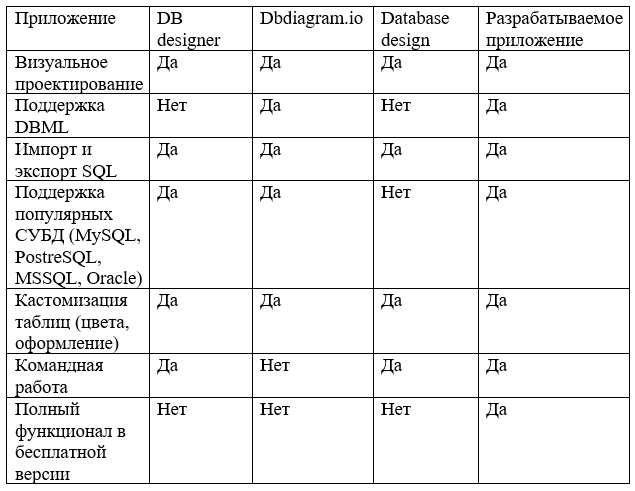
\includegraphics[width=1\textwidth]{analyze.png} % Загружаем изображение и задаем ширину
    \label{fig:analyze} % Метка для ссылок
\end{figure}

\

\textbf{\large 1.3 Функциональные и технические характеристики продукта}
\addcontentsline{toc}{subsection}{1.3.1 Функциональные и технические характеристики продукта}

Разрабатываемое приложение для проектирования баз данных посредством графического интерфейса и DBML обладает рядом функциональных и технических характеристик, которые обеспечивают удобство использоваться и эффективность проектирования.

Приложение должно обеспечивать широкий набор возможностей, необходимых как для индивидуальной работы, так и для совместных проектов:

1. Интерактивное визуальное моделирование.

Приложение предоставляет возможность создавать диаграммы базы данных с помощью интуитивного drag-and-drop редактора.

Пользователь может:

• Создавать таблицы с заданием имен, полей и параметров каждого столбца, включая тип данных, ограничения и дополнительные атрибуты.

• Определять связи между таблицами, устанавливая связи типа один-к-одному, один-ко-многим или многие-ко-многим, что помогает четко структурировать взаимосвязи в базе данных.

• Редактировать элементы диаграммы в реальном времени, перемещая их по виртуальному холсту, что позволяет наглядно представлять и оптимизировать структуру базы данных.

2. Проектирование посредством DBML: приложение должно иметь редактор кода для DBML, при изменении которого будет меняться диаграмма базы данных.

3. Генерация и экспорт кода.

Приложение должно автоматически генерировать рабочий SQL-код, который может быть использован для развертывания базы данных на различных СУБД. Кроме того, должен поддерживаться экспорт описания схемы в формате DBML, что позволяет:

• Документировать структуру базы данных.

• Обеспечить обмен схемами между разработчиками, интегрируя их с другими инструментами и системами.


4. Импорт существующих данных.

Приложение позволит импортировать SQL-дампы или DBML-файлы, что значительно упрощает переход от работы с готовыми проектами к их дальнейшему редактированию. Это позволяет:

• Автоматически распознавать и визуализировать существующую структуру базы данных.

• Вносить изменения в уже разработанные схемы без необходимости начинать проект с нуля.


5. Для поддержки командной работы и управления изменениями приложение предусматривает функционал общего доступа, позволяющий делиться проектами с коллегами или заказчиками, даже если возможность синхронного редактирования может быть ограниченной.

Интерфейс должен быть разработан с прицелом на удобство и простоту использования, обеспечивая интуитивное взаимодействие с пользователем. Основные элементы интерфейса включают:

• Главная рабочая область

• Виртуальный холст, где размещаются все элементы диаграммы, с возможностью масштабирования и перемещения для удобной работы с большими и сложными схемами.

• Поддержка drag-and-drop, позволяющая пользователю легко создавать, перемещать и изменять размеры таблиц и других элементов.

• Набор кнопок и меню для быстрого доступа к основным функциям: создание и удаление таблицы, добавление поля, установка связей, а также экспорт кода.

• Контекстное меню, в котором пользователь может детально настраивать типы данных для выбранного элемента.

• Режим просмотра и редактирования кода

• Возможность редактирования кода вручную, с последующей синхронизацией изменений с визуальной диаграммой.


Для обеспечения стабильной работы приложения и поддержки всех перечисленных функций, предусмотрены следующие минимальные технические характеристики:

 • Операционная система: приложение кроссплатформенное, работает на Windows 10/11, macOS или современных дистрибутивах Linux.
 
 • Процессор: 2-ядерный Intel Core i3 / AMD Ryzen 3 или выше.
 
 • Оперативная память: 4 ГБ.
 
 • Место на диске: 100 МБ (для кэша браузера).
 
 • Браузер: современный браузер, поддерживающий HTML5, CSS3 и JavaScript (Chrome, Yandex, Opera, Edge, Safari), обеспечивающий стабильную и быструю работу интерактивного интерфейса.
 
 • Интернет-соединение: при использовании веб-версии необходимо стабильное высокоскоростное подключение к интернету для синхронной работы с сервером и обеспечения своевременной синхронизации данных.

Функциональные и технические характеристики разрабатываемого приложения направлены на обеспечение удобства и скорости проектирования баз данных. Приложение объединяет в себе мощный визуальный редактор, автоматизированную генерацию кода и инструменты для управления проектами, что делает его универсальным решением для разработки, тестирования и документирования баз данных. Технические характеристики обеспечивают стабильную работу приложения даже на компьютерах с минимальными требованиями.
\\

\textbf{\large 1.4 Требования к системе}
\addcontentsline{toc}{subsection}{1.4 Требования к системе}

\textbf{\large 1.4.1 Бизнес-требования}
\addcontentsline{tocdepth}{subsubsection}{ 1.4.1 Бизнес-требования}

	Цель проекта – предоставить разработчикам, студентам и аналитикам удобный, доступный и функциональный инструмент для визуального проектирования баз данных с поддержкой DBML и генерации SQL-кода.
    
	Коммерческая значимость – приложение может быть использовано как в образовательной среде, так и в профессиональной деятельности для быстрой разработки схем баз данных, что сокращает временные и финансовые издержки.
    
	Конкурентные преимущества – поддержка DBML, бесплатная модель распространения, функции совместной работы и экспорт/импорт SQL.
    
	Целевая аудитория – студенты, фрилансеры, стартапы, разработчики, архитекторы баз данных, аналитики.

\textbf{\large 1.4.2 Функциональные требования }
\addcontentsline{tocdepth}{subsubsection}{ 1.4.2 Функциональные требования}

	1.	Проектирование БД:
    
	•	создание таблиц и полей в визуальном редакторе (drag-and-drop);
    
	•	определение связей между таблицами: 1:1, 1:N, N:1;
    
	•	назначение первичных и внешних ключей;
    
	•	настройка свойств полей (тип, ограничения, nullable и др.).
    
	2.	Работа с кодом:
    
	•	синхронное отображение и редактирование DBML-кода;
    
	•	автоматическая генерация SQL-кода;
    
	•	экспорт и импорт SQL файлов.
    
	3.	Совместная работа:
    
	•	добавление участников в проект;
    
	•	разграничение ролей (owner, editor, viewer);
    
	4.	Управление проектами:
    
	•	создание/удаление/редактирование проектов;
    
	•	клонирование проектов.
    
	5.	Дополнительные функции:
    
	•	подсветка синтаксиса и проверка корректности схемы;
    
	•	автосохранение проекта.
    

\textbf{\large 1.4.3 Нефункциональные требования }
\addcontentsline{tocdepth}{subsubsection}{ 1.4.3 Нефункциональные требования}

	1.	Кроссплатформенность: веб-версия должна работать в современных браузерах;
        
	2.	Производительность:
    
	•	визуальный редактор должен работать без задержек при наличии до 50 таблиц и связей;
    
	•	время генерации SQL – не более 5 секунд при стандартной схеме.
    
	3.	Надежность и отказоустойчивость: автоматическое сохранение проекта;
    
	4.	Безопасность:
    
	•	хеширование паролей пользователей;
    
	•	разграничение прав доступа;
    
	•	защита от XSS и SQL-инъекций.
    
	5.	Удобство интерфейса (UX):
    
	•	поддержка drag-and-drop;
    
	•	тёмная/светлая тема;
    
	•	масштабирование схем.

\textbf{\large 1.4.4 Пользовательские требования }
\addcontentsline{tocdepth}{subsubsection}{ 1.4.4 Пользовательские требования}

	1.	Пользователь должен иметь возможность:
    
	•	зарегистрироваться и войти в систему;
    
	•	создавать и сохранять проекты;
    
	•	добавлять проекты в избранное;
    
	•	проектировать базу через интерфейс или DBML;
    
	•	делиться проектами с другими пользователями;
    
	•	экспортировать проект в SQL.
    
	2.	Пользователь-интерфейс должен быть интуитивно понятным, без необходимости изучения документации.

\textbf{\large 1.4.5 Ограничения}
\addcontentsline{tocdepth}{subsubsection}{ 1.4.5 Ограничения}

	•	Использование только PostgreSQL на серверной стороне.
    
	•	Поддерживаются только реляционные базы данных.
    
	•	Требуется авторизация для доступа к проектам.


\textbf{\large 1.4.6 Требования к интерфейсам}
\addcontentsline{tocdepth}{subsubsection}{ 1.4.6 Требования к интерфейсам}

	Графический интерфейс:
    
	•	редактор диаграмм на виртуальном холсте;
    
	•	панель свойств и инструментов;
    
	•	редактор DBML с подсветкой синтаксиса.
    
	Интерфейс API:
    
	•	REST API для доступа к проектам, таблицам, пользователям;
    
	•	авторизация через токены;
    
	•	ORM (Django ORM) для взаимодействия с PostgreSQL;
    
	•	структура, нормализованная до 3НФ.


\textbf{\large 1.5 Анализ технологий}
\addcontentsline{toc}{subsection}{1.5 Анализ технологий}

\textbf{\large 1.5.1 Выбор языка программирования}
\addcontentsline{tocdepth}{subsubsection}{ 1.5.1 Выбор языка программирования}

Выбор языка программирования является одним из ключевых этапов
разработки приложения, так как он определяет не только скорость и удобство
реализации, но и возможности интеграции с другими технологиями, производительность и поддержку современных функций. В данном разделе проводится анализ языков программирования Python и JavaScript и обоснование их выбора для разработки приложения для проектирования баз данных посредством интерфейса и DBML.

Python обладает рядом преимуществ, которые выделяют его на фоне других языков программирования и делают его особенно привлекательным выбором для разработки серверной логики, десктопных приложений и инструментов для обработки данных. Одним из ключевых достоинств Python является его простота и лаконичность, что позволяет разработчикам писать код быстрее и с меньшим количеством ошибок. Благодаря интуитивно понятному синтаксису, Python существенно снижает порог вхождения в программирование, что особенно важно при работе в команде, где могут быть участники с разным уровнем подготовки.

Кроме того, Python обладает обширной и зрелой экосистемой, включающей тысячи библиотек и фреймворков для самых разных задач. Для веб-разработки существуют такие фреймворки, как Django и Flask, которые позволяют быстро создавать масштабируемые и надежные RESTful API, а для работы с базами данных — SQLAlchemy и Django ORM, обеспечивающие гибкое взаимодействие с различными СУБД. Это значительно упрощает интеграцию с другими системами и ускоряет процесс разработки, поскольку многие типовые задачи уже решены и протестированы сообществом.

Еще одним значительным аспектом является широкая поддержка Python в научном и образовательном сообществе. Благодаря такому сообществу существует масса документации, учебных материалов и примеров, что позволяет не только быстро обучаться, но и эффективно решать сложные задачи. Это особенно важно для проектов, требующих обработки больших объемов данных, генерации кода, анализа и визуализации информации, где Python зарекомендовал себя как один из лучших инструментов.

Если сравнивать Python с такими языками, как Java или C#, то его динамическая типизация и возможность быстрой прототипизации часто дают существенное преимущество на начальных этапах разработки. В Java или C# требуется больше времени на настройку проекта и более строгая структура кода, что может замедлить разработку в условиях быстро меняющихся требований. В то же время Python позволяет быстро тестировать новые идеи, что особенно ценно в стартапах или при разработке инновационных решений, где скорость вывода продукта на рынок играет ключевую роль.

Еще одним важным преимуществом является кроссплатформенность Python. Он работает на большинстве современных операционных систем, включая Windows, macOS и Linux, что делает его универсальным инструментом для создания как веб-приложений, так и десктопных решений. При разработке десктопной версии «DB Builder» Python с использованием таких библиотек, как PyQt или Kivy, позволяет создать стабильное и функциональное приложение, которое одинаково хорошо работает на всех платформах, обеспечивая единообразный пользовательский опыт.

В дополнение к этому, Python поддерживает современные параллельные и асинхронные технологии, что дает возможность эффективно обрабатывать запросы и реализовывать функциональность в реальном времени. Такие технологии, как Django Channels, позволяют создавать приложения с поддержкой WebSocket, что критически важно для разработки инструментов, ориентированных на коллективное редактирование и обмен данными между пользователями в режиме реального времени.

Сравнивая Python с JavaScript на серверной стороне (например, Node.js), можно отметить, что Python часто выигрывает в плане удобства разработки, благодаря более понятному синтаксису и богатому набору библиотек для обработки данных, что особенно важно для проектов, где требуется генерация SQL-кода и работа с DBML. При этом JavaScript, будучи незаменимым для разработки веб-интерфейсов, прекрасно дополняет Python, обеспечивая создание динамичных и интерактивных пользовательских интерфейсов. Такой подход позволяет разделить обязанности между серверной и клиентской частями, что повышает модульность и масштабируемость всего приложения.

Также Python активно используется в области машинного обучения и аналитики данных, что открывает дополнительные перспективы для интеграции возможностей искусственного интеллекта и предиктивной аналитики в будущем. Это может быть особенно полезно для расширения функциональности, например, для автоматического анализа структур баз данных, рекомендаций по оптимизации схем или выявления потенциальных проблем в дизайне базы данных.

Таким образом, выбор Python обусловлен его простотой, гибкостью, широкой поддержкой и возможностями быстрого прототипирования, что позволяет создавать надежные, масштабируемые и легко поддерживаемые решения. Все эти факторы делают Python оптимальным выбором для реализации серверной логики, обработки данных и создания десктопной версии приложения, особенно в сочетании с JavaScript, который обеспечивает создание современного, интуитивно понятного веб-интерфейса.

\textbf{\large 1.5.2 Анализ фреймворков}
\addcontentsline{tocdepth}{subsubsection}{ 1.5.2 Анализ фреймворков}

Для разработки веб-версии приложения необходимо выбрать подходящий фреймворк, который обеспечит баланс между производительностью, удобством разработки и возможностями масштабирования. В Python существует несколько популярных фреймворков для веб-разработки, среди которых наиболее распространены Django и Flask. Оба фреймворка широко используются в индустрии, но имеют принципиально разные подходы к разработке, что делает их выбор важным этапом проектирования архитектуры приложения.

1. Анализ Python-фреймворков для серверной части.

Django — это мощный, полнофункциональный веб-фреймворк, который следует принципу “батарейки в комплекте”. Он предоставляет разработчикам встроенные решения для работы с базами данных через ORM (Object-Relational Mapping), управление пользователями, аутентификацию, админ-панель, систему шаблонов и многое другое. Благодаря своей структуре и четко организованному паттерну Model-View-Template (MVT), Django позволяет разрабатывать сложные веб-приложения с минимальными затратами на рутинные задачи.

Одним из главных преимуществ Django является его высокая степень безопасности. Встроенные механизмы защиты от SQL-инъекций, XSS- и CSRF-атак, а также встроенная система аутентификации делают его надежным выбором для веб-приложений, работающих с конфиденциальными данными. Это особенно важно для проекта, связанного с проектированием баз данных, так как потенциальные утечки могут привести к серьезным последствиям.

Еще одним важным фактором является высокая масштабируемость. Django позволяет быстро расширять функциональность приложения, а его архитектура способствует разработке сложных проектов, где требуется четкое разделение логики, данных и представления. Встроенная система кэширования и возможность интеграции с различными базами данных (PostgreSQL, MySQL, SQLite и другими) позволяют адаптировать фреймворк под любые задачи.

Однако у Django есть и недостатки. Из-за своей монолитной структуры он может быть избыточным для небольших или простых приложений, где требуется минимальный набор функционала. Кроме того, его высокая абстракция и автоматизация некоторых процессов могут снизить гибкость разработки, если необходимо тонко настраивать приложение.

Flask, в отличие от Django, является легковесным микрофреймворком, который предоставляет только базовые инструменты для разработки веб-приложений. Он не включает в себя встроенную ORM, систему авторизации или админ-панель, но благодаря своей минималистичной архитектуре позволяет разработчикам выбирать только необходимые библиотеки и компоненты, что делает его более гибким.

Одним из главных преимуществ Flask является его простота и легкость. Он не навязывает строгую структуру проекта, что делает его отличным выбором для небольших приложений, API-сервисов или микросервисной архитектуры. Flask также хорошо интегрируется с асинхронными технологиями и может использоваться совместно с библиотеками для WebSocket’ов, что позволяет создавать более интерактивные приложения.

Еще одним плюсом Flask является его производительность. Благодаря отсутствию избыточных компонентов он работает быстрее, чем Django, и потребляет меньше ресурсов, что может быть критически важно при развертывании на серверах с ограниченными ресурсами.

Однако Flask требует больше времени на настройку и внедрение некоторых функций. Например, если необходимо добавить ORM, систему аутентификации или админ-панель, разработчику придется использовать сторонние библиотеки и самостоятельно интегрировать их в проект. Это может увеличить сложность разработки и потребовать дополнительных усилий по поддержке кода.

Учитывая специфику проекта, Django представляется оптимальным выбором для реализации серверной части. Встроенная ORM позволит эффективно управлять схемами баз данных, а развитая экосистема обеспечит быстрый старт и возможность дальнейшего масштабирования. Дополнительные инструменты, такие как встроенная панель администратора, могут быть полезны для управления пользователями и их проектами, а высокий уровень безопасности обеспечит защиту данных.

Однако Flask может быть рассмотрен в качестве альтернативы, если впоследствии потребуется разработка легковесного API для интеграции с другими сервисами.

2. Анализ JavaScript-фреймворков для клиентской части

Среди существующих решений для визуализации данных выделяется несколько ключевых вариантов. Универсальные библиотеки типа D3.js предоставляют широкие возможности кастомизации, однако требуют значительных трудозатрат на реализацию базовой функциональности. Специализированные фреймворки, такие как mxGraph и JointJS, предлагают готовые компоненты для работы с диаграммами, но обладают ограниченной гибкостью при работе со сложными структурами данных.

Библиотека Go.js представляет собой оптимальный баланс между функциональностью и удобством разработки. Ее архитектура специально разработана для создания интерактивных диаграмм с поддержкой сложных операций. Встроенные механизмы обработки пользовательского ввода, включая перетаскивание элементов и изменение связей, значительно сокращают время разработки по сравнению с альтернативными решениями.

Производительность Go.js при работе с крупными схемами становится решающим фактором выбора. Библиотека использует оптимизированные алгоритмы рендеринга, что обеспечивает плавную работу интерфейса даже при визуализации сложных структур с десятками взаимосвязанных таблиц. Это критически важно для профессионального инструмента проектирования баз данных.

Для реализации текстового редактора схем рассматриваются несколько вариантов. CodeMirror и Ace Editor представляют собой легковесные решения с базовой функциональностью, однако их возможности работы с языками описания структур данных ограничены. Monaco Editor, являясь основой Visual Studio Code, предлагает полный набор профессиональных инструментов для работы с кодом.

Глубокая интеграция Monaco Editor с языковыми серверами обеспечивает продвинутую подсветку синтаксиса, автодополнение и статический анализ кода для DBML и SQL. Эти функции существенно повышают продуктивность работы пользователей при редактировании схем баз данных. Поддержка TypeScript в Monaco Editor также соответствует выбранному технологическому стеку разработки.

При сравнении комбинации Go.js и Monaco Editor с альтернативными подходами выявляются существенные преимущества выбранного решения. Использование универсальных фреймворков с дополнительными библиотеками приводит к усложнению архитектуры и увеличению времени разработки. Специализированные же инструменты предоставляют готовую функциональность, оптимизированную под конкретные задачи проектирования баз данных.

Важным аспектом является возможность глубокой интеграции между визуальным и текстовым представлениями схемы. Выбранные технологии позволяют реализовать двустороннюю синхронизацию изменений, что создает целостную среду разработки. Пользователи получают возможность свободно переключаться между графическим и текстовым режимами работы без потери данных или согласованности представления.

Таким образом, сочетание Django для серверной части и Go.js с Monaco Editor для клиентской представляет собой наиболее обоснованное решение для создания инструмента проектирования баз данных. Сочетание этих технологий обеспечивает необходимый уровень функциональности, производительности и удобства разработки, позволяя создавать продукт, соответствующий современным требованиям веб-приложений.

\

\textbf{\large 1.6 Выводы}
\addcontentsline{toc}{subsection}{1.6 Выводы}

Проведенный анализ предметной области подтвердил актуальность разработки приложения для визуального проектирования баз данных и генерации SQL-кода посредством DBML. Несмотря на наличие множества инструментов для визуального моделирования баз данных, существующие решения имеют ряд ограничений, таких как высокая стоимость, ограниченный функционал в бесплатных версиях и недостаточные возможности для командной работы.

Особенно остро проблема стоит для студентов, начинающих разработчиков и небольших команд, которым необходимо удобное, доступное и функциональное решение для проектирования баз данных. В ходе анализа были рассмотрены существующие инструменты, такие как DB Designer, Dbdiagram.io и Database-design. Они обладают рядом полезных функций, включая визуальное моделирование, экспорт в SQL, поддержку различных СУБД и возможность совместной работы. Однако каждый из них имеет свои недостатки, среди которых ограничения в бесплатных версиях, отсутствие поддержки DBML, проблемы с одновременным редактированием и невозможность работы без подключения к интернету.

На основании проведенного анализа можно сделать вывод о необходимости разработки нового инструмента для проектирования баз данных, который объединит в себе преимущества существующих решений и устранит их основные недостатки. Разрабатываемое приложение должно предоставить пользователям удобный интерфейс для визуального моделирования баз данных, поддержку DBML, возможность экспорта SQL, а также функции командной работы.

Таким образом, анализ предметной области подтвердил актуальность разработки нового инструмента для проектирования баз данных, который станет доступной альтернативой существующим решениям и обеспечит пользователей широким набором функций для эффективной работы.